\chapter{Introducción}
\label{chap:Introduction}
\Quote{Es siempre sabio mirar adelante, pero difícil mirar más allá de lo que puedes.}{Winston Churchill (1874--1965)} 

\Abstract{Este primer capítulo introduce a la visión artificial y demuestra el gran interés otorgado por la comunidad científica en este área. También se muestra la motivación de este proyecto, así como sus objetivos y se desarrolla la estructura del mismo.}

Los orígenes de la visión artificial surgieron en 1960 como sistemas para el reconocimiento de patrones y centrados en su posible implantación en el sector industrial debido a la gran cantidad de tareas repetitivas fácilmente automatizables \citep{50years}. A pesar de la carencia de los recursos en su momento, pero debido al gran interés del mercado estos siguieron siendo desarrollados y poco a poco implantados. Una de las primeras empresas en implantar estos sistemas fue Hitachi Labs en 1964 en Japón \cite{50years}.

Desgraciadamente estos primeros desarrollos carecían de precisión y tenían una tasa de acierto del 95\% (no se consideró suficiente para su implementación en una línea de producción). Pero esto se vería resuelto en los años venideros de forma que en la década de los 70 estos sistemas pasaron a formar parte de una gran parte del sector industrial. Un claro ejemplo fue la automatización de la producción de transistores con semiconductores en 1974 por Hitachi ya que, debido a su complejidad, esta tarea no podía ser llevada a cabo por humanos \cite{hitachi}

Gracias al desarrollo de nuevas tecnologías en el sector fotográfico, se desarrollaron nuevos métodos para la captura de imágenes que permitían mejorar la calidad de estas, así como la captura de nueva información como la dimensión del objeto y su distancia respecto a la cámara. También se consiguió un incremento significativo de la capacidad computacional de los nuevos ordenadores. Y es debido a estos dos avances que se ha permitido el desarrollo de nuevos y más sofisticados sistemas de reconocimiento de objetos. Estos nuevos sistemas tienen una gran variedad de usos como conducción autónoma \cite{AIvehicle}, sistemas de seguridad autónomos \cite{AIsecurity}, control forestal \cite{AIdrones}, etc.

En la actualidad se pueden distinguir dos tipos de visión artificial en función de sus capacidades de adaptación. En primer lugar, se encuentran los sistemas más simples empezados a desarrollar en 1960 y que han sido programas para cumplir un único objetivo bajo unas circunstancias dadas. Estos son los menos potentes ya que no se adaptan y no saben reaccionar ante un cambio, pero son los más fáciles de desarrollar. Además, en espacios controlados pueden llegar a dar mejores resultados que sistemas más complejos y avanzados \cite{ABB}. Por ello se van a emplear estos sistemas para el desarrollo de este proyecto \cite{industry4}.

Por otro lado, con el desarrollo de las redes neuronales y de inteligencias artificiales, se están desarrollando sistemas capaces de aprender y adaptarse a la situación a base de prueba y error. Se trata de sistemas muy modernos todavía en desarrollo que prometen traer avances como la conducción autónoma, detección de emociones en humanos, etc. Estos sistemas necesitan de grandes cantidades de bases de datos de las que aprender. Pero debido a la capacidad de cálculo necesaria para entrenarlos, se escapan del principal objetivo de este proyecto.

El fin de este proyecto es la mejora de un sistema de reconocimiento y recogida de piezas LEGO con un brazo robótico. Para ello se parte de un proyecto previo desarrollado por Ana Berjón \cite{TFGAna} y un robot dotado con una cámara RGB-D. El objetivo es mejorar 3 sistema actual y hacerlo más robustos ante cambios en la escena (iluminación, disposición de las piezas, etc.).

\section{Motivación}
\label{sec:Motivación}
La industria avanza a un ritmo constante y cada día es más necesario la implantación de sistemas robóticos para poder llevar a cabo tareas que los humanos no podemos. Al dotar a estos sistemas de inteligencia y un sistema de visión artificial, se consigue que se pueda adaptar mejor al entorno y se evite tener que reprogramar los robots con cada cambio de las condiciones de operación. Avanzamos hacia una sociedad en la que los robots serán la principal mano de obra y para llegar a ese objetivo es necesario invertir y desarrollar más los sistemas actuales. Por ello se ha propuesto como proyecto la integración de un sistema de visión artificial en un brazo robótico. Con este proyecto se podrá modernizar las instalaciones de ICAI y aumentar las capacidades de los robots actuales, así como instruir a futuros alumnos sobre la visión artificial.


\section{Objetivos}
\label{sec:Objetivos}
Este proyecto parte del trabajo previo de Ana Berjón Valles y Lucia Díaz García y el objetivo es mejorar el sistema actual y dotarlo de nuevas capacidades. Para ello se ha mejorado la respuesta del sistema ante cambios de iluminación y de escena mediante el uso de redes neuronales. Gracias al uso de estas redes también se ha mejorada la robustez y rapidez del sistema.

El anterior sistema presentaba problemas de conexión y por ello en ocasiones la cámara dejaba de responder o las imágenes eran corrompidas. Como objetivo de este proyecto se ha decidido mejorar la conexión con la cámara. Para ello se ha diseñado desde cero un nuevo \textit{driver} de la cámara que permite una conexión más rápida y estable sin imágenes corrompidas. Este mismo \textit{driver} se emplea también para la adquisición de la imagen de profundidad. Además, se ha implantado un método para corregir la distorsión y diferencia de enfoque entre la imagen de color y la de profundidad permitiendo así realizar medidas más precisas.

El análisis de la profundidad ha sido perfeccionado con el fin de mitigar el efecto causado por los reflejos. Para ello se ha diseñado una nueva forma de trabajo y análisis así como la opción de calibración para la profundidad.

Mejora del sistema de cálculo de la orientación de una pieza. Se ha mejorado el anterior sistema de forma que siempre pueda detectar el ángulo y se ha reducido el error cometido. Para ello se realiza un análisis mas exhaustivo de la pieza. Además, se han desarrollado redes neuronales para llevar a cabo esta tarea.

Para mejorar las instalaciones de la universidad y dotar de más capacidad al resto de robots del laboratorio se han generalizado en todo lo posible los algoritmos empleados para permitir así su implantación en otros sistemas.

Se han planteado más objetivos adicionales para realizar en el transcurso de este proyecto pero debido a una pandemia no se ha podido tener suficiente acceso al robot y por lo tanto han tenido que ser retrasados. Estos son el uso de piezas de LEGO dobles y el establecimiento de una comunicación bidireccional entre el brazo robótico y MATLAB. En su lugar, se ha desarrollado en mayor profundidad las redes neuronales.

\section{Herramientas}
\label{sec:Herramientas}
Para el desarrollo del proyecto se requiere de:

	\begin{itemize}
	\item Brazo robótico ABB IRB120 \cite{IRB120} y RobotStudio 2019.5 \cite{RobotStudio}.
	\item Cámara Intel RealSense D435 \cite{IntelD435} y Wrapper de MATLAB para Intel Realsense \cite{Wrapper}.
	\item MATLAB 2019 B con los siguientes paquetes:
		\begin{itemize}
			\item Deep Learning Toolbox Model for AlexNet Network.
			\item Deep Learning Toolbox Model for VGG-16 Network.
			\item Instrument Control Toolbox.
			\item Deep Learning Toolbox.
			\item Bioinformatics Toolbox.
			\item Computer Vision Toolbox.
			\item Parallel Computing Toolbox.
			\item Image Processing Toolbox.
			\item Matlab Support Package for USB Webcams.
			\item Statistics and Machine Learning Toolbox.
		\end{itemize}
	\end{itemize}

\section{Arquitectura del sistema}
\label{sec:Arquitectura}
El sistema se compone de tres elementos claves: un brazo robótico para poder interactuar con las piezas, una cámara montada sobre el brazo robótico para la captura de imágenes y MATLAB para el procesamiento de las imágenes y la toma de decisiones. Es necesario que estos tres elementos funcionen correctamente y estén comunicados entre sí. Como ya se ha mencionado, todas las comunicaciones y decisiones son tomadas por el ordenador y transmitidas a la cámara por conexión USB y al brazo robótico mediante un socket TCP/IP.

	\begin{figure}[ht]
		\centering
		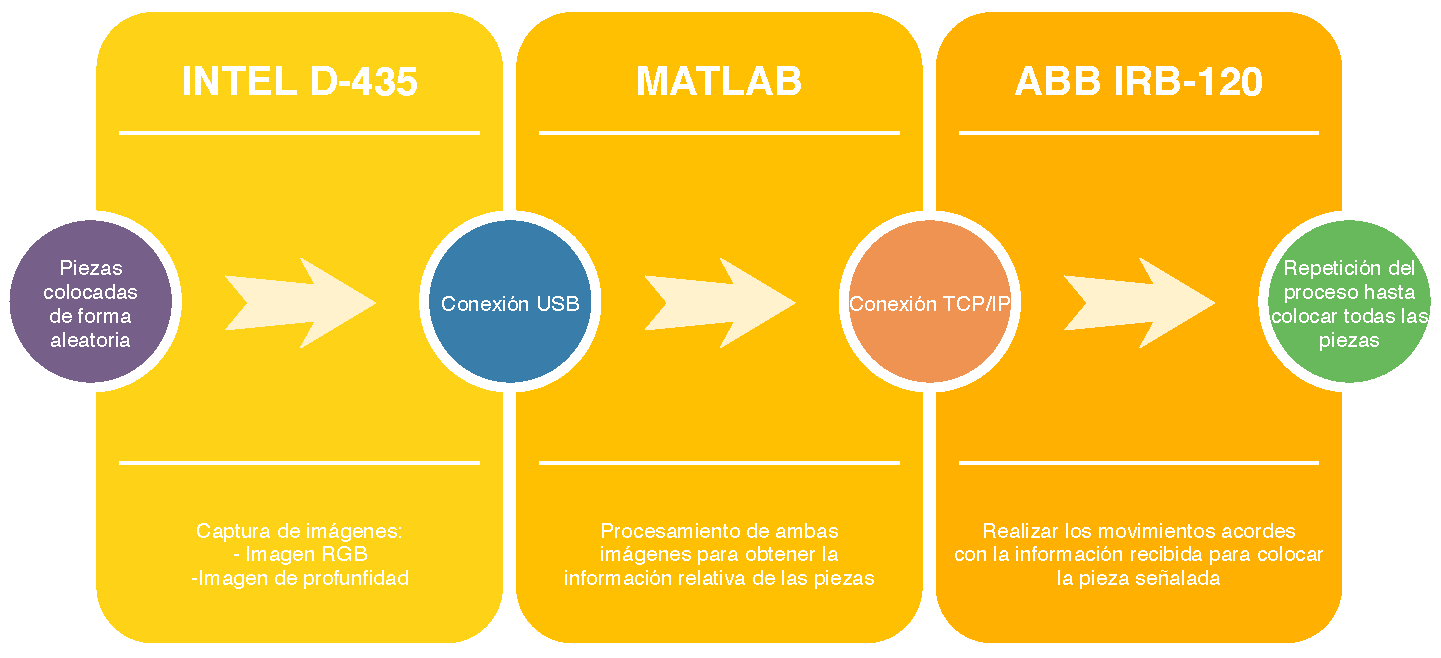
\includegraphics[width=0.9\textwidth]{Introduccion/Esquema_arquitectura.pdf}
		\caption{Esquema de la arquitectura del sistema}
		\label{fig:Arq1}
		\vspace{-5pt}
	\end{figure}

A continuación, se va a detallar todo el proceso desde el arranque del sistema hasta el final del mismo y se analizarán cada una de las etapas que constituyen el proceso. Este se puede ver gráficamente en \autoref{fig:Arq2}. Al arrancar el programa, el primero proceso es la calibración del sistema. Para ello se inicia la conexión de la cámara y se le da tiempo para permitir que se ajuste a las condiciones lumínicas del momento. Acto seguido, se tomará una imagen de profundidad que se usará como referencia de suelo para calcular alturas. Por último, se carga en memoria la red neuronal a emplear para la detección de las piezas.

Una vez iniciado el sistema se puede comenzar a identificar piezas para su futura colecta. El primer paso es la captura de una imagen de color y otra de profundidad, para ello es necesario que el robot se encuentre en su posición de captura de imágenes. Una vez situado en la posición de captura, se toma la imagen y comienza el procesamiento de las imágenes. Para ello existen diferentes sistemas de detección que se explicarán más adelante, pero el objetivo de todos ellos es el mismo, identificar la pieza, su orientación y su altura. Todo este proceso se lleva a cabo con MATLAB y se realiza por etapas. La primera etapa consiste en la detección de la pieza en la imagen. Para ello como se desarrollará más delante, se van a emplear diversos detectores de objetos. Una vez esta ha sido detectada se deben de extraer sus características. Estas consisten en la extracción de su orientación y de su altura. Para la extracción de la orientación existen diversos métodos que se desarrollaran más adelante pero el objetivo es obtener el ángulo de la pieza respecto a un eje del robot para así estimar cuanto debe de rotar este. El análisis de la altura se hace con la ayuda de la imagen de profundidad. Al comparar la altura de la pieza frente al nivel del suelo de la calibración se puede estimar la altura de la pieza y el número de piezas de LEGO apiladas.

Tras obtener las coordenadas de la pieza en la imagen, su orientación y altura, se transforman estas coordenadas en píxeles a coordenadas respecto al robot. Una vez obtenidas todas las coordenadas, estas son mandadas al robot para la recolección de las piezas y su disposición en una región de recolección determinada. Una vez terminado este proceso, el robot volverá a la posición de captura y se volverá a iniciar todo el proceso hasta que se haya recolectado todas las piezas.

	\begin{figure}[ht]
		\centering
		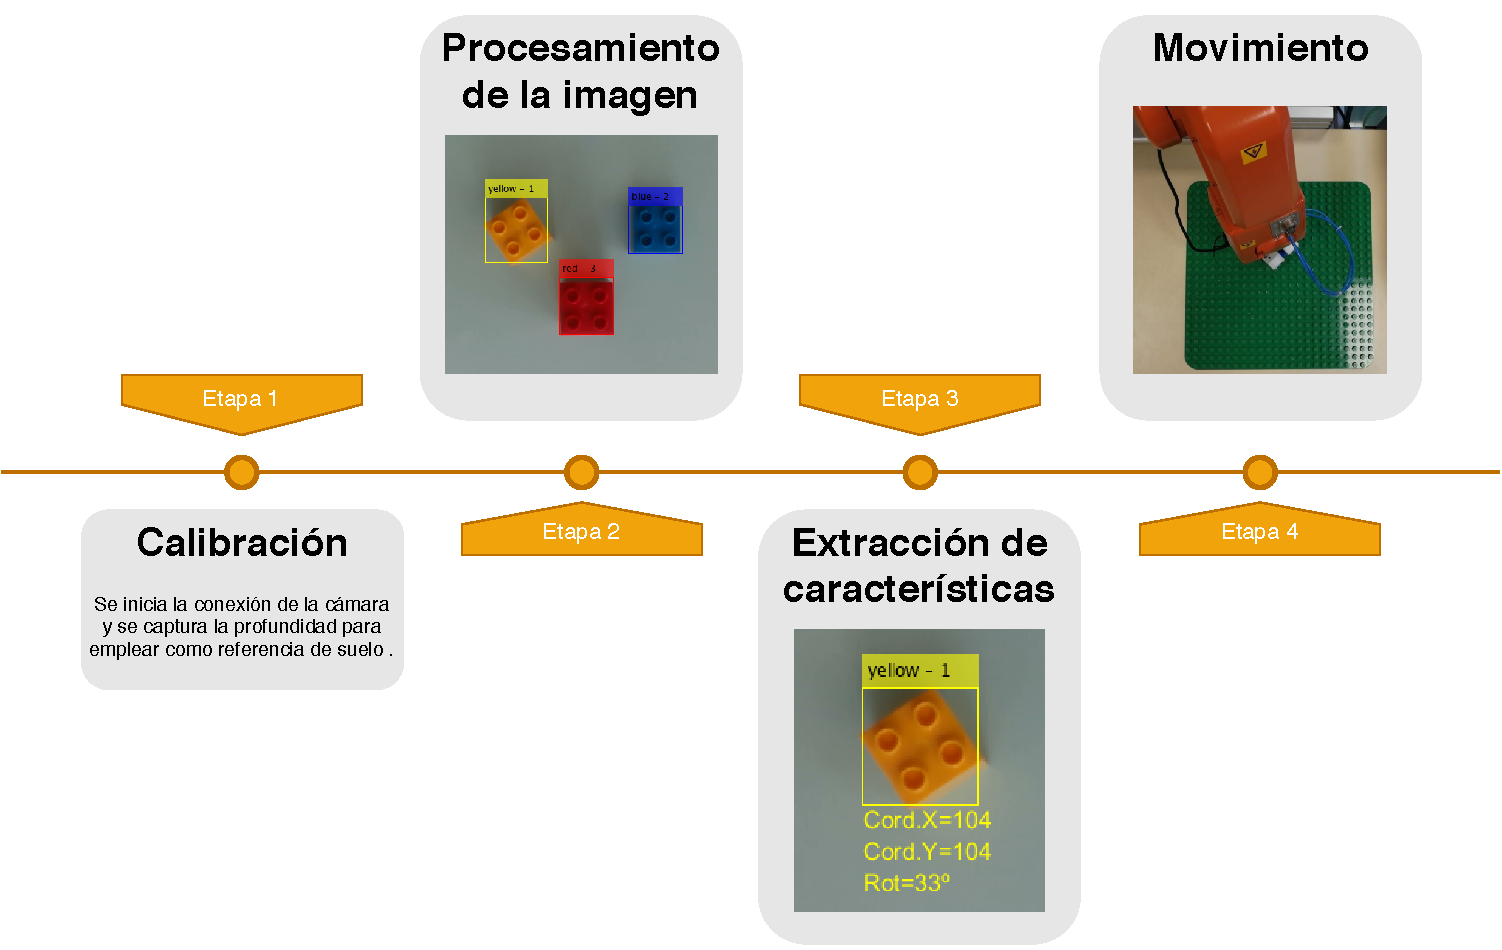
\includegraphics[width=0.9\textwidth]{Introduccion/Diagrama_arquitectura.pdf}
		\caption{Diagrama de las etapas del sistema}
		\label{fig:Arq2}
		\vspace{-5pt}
	\end{figure}

\section{Organización del documento}
\label{sec:Organización}
La estructura de este documento se asemeja a la seguida durante el desarrollo de este proyecto. De esta forma se asegura una buena conexión entre los diversos capítulos y sus respectivas secciones. La memoria se distribuye en 9 capítulos, siendo el presente el primero de ellos, que introduce el problema del proyecto y la motivación del mismo. El siguiente capítulo contiene la revisión de la literatura, en este capítulo se contextualiza el proyecto y se desarrollan todos los temas tratados en este proyecto.

Una vez introducido y contextualiza el proyecto se comienza a desarrollar las herramientas y métodos necesarios. Esto comienza por el perfeccionamiento del trabajo desarrollado por Ana Berjón Valles y Lucia Díaz García. Esto se lleva a cabo en el tercer capítulo con la segmentación con mascaras de color. El cuarto capítulo introduce las redes neuronales y sus capacidades. En este capítulo también se desarrollaran dos clasificadores para su posterior reaprovechamiento en el capítulo 5. En el quinto capítulo se desarrollan diversos métodos para la segmentación con redes neuronales y se evalúan dichos métodos. El sexto capítulo trata sobre la extracción del resto de atributos de las piezas de LEGO, esto incluye la obtención de la altura así como la estimación de la orientación. Una vez desarrollados todos los métodos para la extracción de atributos y la detección, se compararan y contrastaran resultados en el séptimo capítulo.

Por último, en los dos últimos capítulos se desarrollará una conclusión final y completa del proyecto así como futuras vias de desarrollo y de mejora de este proyecto. Esto se llevará a cabo en los capítulos octavo y noveno respectivamente.